\section{Generators}\label{generators}

\subsection{Internal Combustion Engine}\label{internal-combustion-engine}

The engine-driven generator model was originally developed for the BLAST program and was subsequently adapted for use in EnergyPlus. The model uses the following set of equations all of which are quadratic fits to the PLR (Part Load Ratio) of the generator.~ The coefficients must be derived from manufacturers data.

\begin{equation}
\frac{{electric~energy~output}}{{fuel~energy~input}} = \frac{{electric~energy~output}}{{\left( {{{\dot m}_{fuel}}\left\{ {kg/s} \right\} \cdot LHV\left\{ {J/kg} \right\}} \right)}} = {a_1} + {a_2}PLR + {a_3}PL{R^2}
\end{equation}

The electrical load and engine generator nominal load capacity are used to compute the part load ratio.

\begin{equation}
PLR = \frac{{Electric~energy~output}}{{nominal~generating~capacity}}
\end{equation}

The exhaust gas temp and flow rate are used if a stack heat exchanger is used to recover waste heat from the exhaust.~ This temperature is the inlet temperature to the heat exchanger which is modeled in a UA-effectiveness form:

\begin{equation}
\frac{{Total~Exhaust~heat}}{{fuel~energy~input}} = \frac{{Total~Exhaust~heat}}{{\left( {{{\dot m}_{fuel}}\left\{ {kg/s} \right\} \cdot LHV\left\{ {J/kg} \right\}} \right)}} = {d_1} + {d_2}PLR + {d_3}PL{R^2}
\end{equation}

\begin{equation}
\frac{{Exhaust~Gas~Temp~\left\{ K \right\}}}{{fuel~energy~input}} = \frac{{Exhaust~Gas~Temp\,\,\left\{ K \right\}}}{{\left( {{{\dot m}_{fuel}}\left\{ {kg/s} \right\} \cdot LHV\left\{ {J/kg} \right\}} \right)}} = {e_1} + {e_2}PLR + {e_3}PL{R^2}
\end{equation}

The exhaust flow rate is then calculated as:

\begin{equation}
{\dot m_{exhaust}} = \frac{{Total~Exhaust~heat}}{{C{p_{exhaust}} \cdot \left( {{T_{exhaust}} - {T_{reference}}} \right)}}
\end{equation}

where T\(_{reference}\) is the reference temperature for the fuel lower heating value (given as 25\(^{\circ}\)C in manufacturer's data) and:

\begin{equation}
{T_{stack}} = {T_{DesignMinExhaust}} + {\frac{{\left( {{T_{exhaust}} - {T_{DesignMinExhaust}}} \right)}}{{{\rm{exp}}\left( {\frac{{{\rm{UA}}}}{{{{{\rm{\dot m}}}_{{\rm{exhaust}}}}C{p_{exhaust}}}}} \right)}}^2}
\end{equation}

Finally heat recovered from the lube oil and the water jacket are accounted for as follows:

\begin{equation}
\frac{{Recoverable~jacket~heat}}{{fuel~energy~input}} = \frac{{Recoverable~jacket~heat}}{{\left( {{{\dot m}_{fuel}}\left\{ {kg/s} \right\} \cdot LHV\left\{ {J/kg} \right\}} \right)}} = {b_1} + {b_2}PLR + {b_3}PL{R^2}
\end{equation}

\begin{equation}
\frac{{Recoverable~lube~oil~heat}}{{fuel~energy~input}} = \frac{{Recoverable~lube~oil~heat}}{{\left( {{{\dot m}_{fuel}}\left\{ {kg/s} \right\} \cdot LHV\left\{ {J/kg} \right\}} \right)}} = {c_1} + {c_2}PLR + {c_3}PL{R^2}
\end{equation}

The manufacturer must supply the recoverable water jacket heat, lube oil heat and exhaust heat and associated fuel consumption for a range of load conditions.~ This data is then fit to the PLR to obtain the fifteen a,b,c,d, and e coefficients.

\subsection{Turbine Generator}\label{turbine-generator}

The combustion turbine generator model was originally developed for the BLAST program and was subsequently adapted for use in EnergyPlus. The model uses the following set of equations all of which are equation fits to the PLR (Part Load Ratio) of the generator and the entering air temperature. The coefficients must be derived from manufacturers data. For electric power generated in Watts, the fuel input rate is calculated in J/s.

\begin{equation}
\frac{{{\rm{fuel~energy~input~rate}}}}{{{\rm{electric~power~output}}}} = \left[ {{a_1} + {a_2}PLR + {a_3}PL{R^2}} \right] * \left[ {{b_1} + {b_2}\Delta T + {b_3}\Delta {T^2}} \right]
\end{equation}

The electrical load and engine generator nominal load capacity are used to compute the part load ratio.

\begin{equation}
PLR = \frac{{{\rm{Electric~energy~output}}}}{{{\rm{nominal~generating~capacity}}}}
\end{equation}

The temperature difference shows the deviation of ambient air temperature from the manufacturers design air temperature.

\begin{equation}
\Delta T = {T_{air}} - {T_{design}}
\end{equation}

A second curve fit calculates the exhaust temperature (C) by multiplying the exhaust temperature (C) for a particular part load by a correction factor based on the deviation from design temperature.

\begin{equation}
{{\rm{T}}_{exhaust}} = \left[ {{c_1} + {c_2}PLR + {c_3}PL{R^2}} \right] * \left[ {{d_1} + {d_2}\Delta T + {d_3}\Delta {T^2}} \right]
\end{equation}

The exhaust gas temp is used if a stack heat exchanger is used to recover waste heat from the exhaust.~ This temperature is the inlet temperature to the heat exchanger which is modeled in a UA-effectiveness form:

\begin{equation}
{T_{stack}} = {T_{DesignMinExhaust}} + {\frac{{\left( {{T_{exhaust}} - {T_{DesignMinExhaust}}} \right)}}{{{\rm{exp}}\left( {\frac{{{\rm{UA}}}}{{{{{\rm{\dot m}}}_{{\rm{exhaust}}}}C{p_{exhaust}}}}} \right)}}^2}
\end{equation}

Where the design minimum exhaust temperature is a user input to the model and the exhaust mass flow rate and the UA are fit from manufacturers data as follows:

\begin{equation}
UA = {e_3}{{(Nominal~Generating~Capacity)}^{e4}}
\end{equation}

\begin{equation}
\frac{{{\rm{exhaust~gas~flow~rate}}}}{{{\rm{Nominal~Generating~Capacity}}}} = \left[ {{f_1} + {f_2}\Delta T + {f_3}\Delta {T^2}} \right]
\end{equation}

Finally, heat recovered from the lube oil is accounted for as follows:

\begin{equation}
\frac{{{\rm{Recoverable~lube~oil~heat}}}}{{{\rm{electric~power~generated}}}} = {g_1} + {g_2}PLR + {g_3}PL{R^2}
\end{equation}

\subsection{Microturbine Generator}\label{microturbine-generator}

Microturbine generators are small combustion turbines that produce electricity on a relatively small scale (e.g., 25kW to 500kW). This model uses nominal performance at reference conditions along with several modifier curves to determine electrical power output and fuel use at non-reference conditions. The modifier curve coefficients must be derived from manufacturers data. Standby and ancillary power can also be taken into account.

Exhaust air energy recovery for heating water can be also be modeled. Similar to electrical power output, thermal power (heat recovery to water) output is calculated using nominal performance at reference conditions with modifier curves to account for variations at non-reference conditions. The ElectricLoadCenter:Generators and ElectricLoadCenter:Distribution objects are used to define the availability and control of the electric generators included in the simulation (ref. ElectricLoadCenter:Generators and ElectricLoadCenter:Distribution).

For each simulation time step that the generator is being asked to operate (i.e., produce electrical power as determined by the ElectricLoadCenter), the full load electrical output of the generator is determined using the user-defined reference electrical power output along with a bi-quadratic modifier curve to account for differences in the combustion air inlet temperature and elevation for the current simulation time step compared to the reference temperature and elevation (i.e., the modifier curve should evaluate to 1.0 at the reference combustion air inlet temperature and reference elevation).

\begin{equation}
{P_{Elec,Full~Load}} = {P_{Elec,Ref}}\left( {PowerFTempElev} \right)
\end{equation}

\begin{equation}
PowerFTempElev = {a_1} + {a_2}\left( {{T_{a,i}}} \right) + {a_3}{\left( {{T_{a,i}}} \right)^2} + {a_4}\left( {Elev} \right) + {a_5}{\left( {Elev} \right)^2} + {a_6}\left( {{T_{a,i}}} \right)\left( {Elev} \right)
\end{equation}

where:

\({P_{Elec,Full~Load}}\) is the full load electrical power output (W)

\({P_{Elec,Ref}}\) is the reference electrical power output, user input (W)

\(PowerFTempElev\) is the user-defined Electric Power Modifier Curve (function of temperature and elevation) evaluated at the current combustion air inlet temperature and elevation

\({T_{a,i}}\) is the combustion air inlet temperature (\(^{\circ}\)C)

\(Elev\) is the elevation (m). This value obtained from the Location object or the weather file.

The full load electrical power output of the generator is then checked against the minimum and maximum full load electrical power outputs specified by the user:

\begin{equation}
{P_{Elec,Full~Load}} = MIN\left( {{P_{Elec,Full~Load}},{P_{FL,Max}}} \right)
\end{equation}

\begin{equation}
{P_{Elec,Full~Load}} = MAX\left( {{P_{Elec,Full~Load}},{P_{FL,Min}}} \right)
\end{equation}

where:

\({P_{FL,Max}}\) is the maximum Full Load Electrical Power Output, user input (W)

\({P_{FL,Min}}\) is the minimum Full Load Electrical Power Output, user input (W).

The actual (operating) electrical power output from the generator is determined next based on the load requested by the Electric Load Center, the generator's minimum and maximum part-load ratios, and the ancillary power.

\begin{equation}
{P_{Elec,Operating}} = MAX\left( {0.0,\left( {Load + {P_{Ancillary}}} \right)} \right)
\end{equation}

\begin{equation}
{P_{Elec,Operating}} = MIN\left( {{P_{Elec,Operating}},{P_{Elec,Full~Load}}} \right)
\end{equation}

\begin{equation}
\begin{array}{l}
~~~~IF~( {P_{Elec,Full~Load}} > 0 )~THEN \\
~~~~~~~~PLR = {P_{Elec,Operating}} / {P_{Elec,Full~Load}} \\
~~~~~~~~PLR = MIN( PLR, PLR_{max} ) \\
~~~~~~~~PLR = MAX( PLR, PLR_{min} ) \\
~~~~ELSE \\
~~~~~~~~PLR = 0 \\
~~~~END IF
\end{array}
\end{equation}

\begin{equation}
{P_{Elec,Operating}} = {P_{Elec,Full~Load}} * PLR
\end{equation}

where:

\({P_{Elec,Operating}}\) is the actual (operating) electrical power output (W)

\(Load\) is the electrical power output being requested by the Electric Load Center (W)

\({P_{Ancillary}}\) is the ancillary power, user input (W)

\(PLR\) is the part-load ratio of the electric generator

\(PL{R_{max}}\) is the maximum part-load ratio of the electric generator (i.e., the maximum value for the independent variable {[}PLR{]} defined in the Curve:Quadratic or Curve:Cubic object for the Electrical Efficiency Modifier Curve {[}function of part-load ratio{]})

\(PL{R_{min}}\) is the minimum part-load ratio of the electric generator (i.e., the minimum value for the independent variable {[}PLR{]} defined in the Curve:Quadratic or Curve:Cubic object for the Electrical Efficiency Modifier Curve {[}function of part-load ratio{]}).

The generator's electrical efficiency is then calculated based on the user-specified reference electrical efficiency (lower heating value {[}LHV{]} basis) and two electrical efficiency modifier curves.

\begin{equation}
ElecEfficiencyFTemp = {b_1} + {b_2}\left( {{T_{a,i}}} \right) + {b_3}{\left( {{T_{a,i}}} \right)^2}~~or~~{b_1} + {b_2}\left( {{T_{a,i}}} \right) + {b_3}{\left( {{T_{a,i}}} \right)^2} + {b_4}{\left( {{T_{a,i}}} \right)^3}
\end{equation}

\begin{equation}
ElecEfficiencyFPLR = {c_1} + {c_2}\left( {PLR} \right) + {c_3}{\left( {PLR} \right)^2}~~or~~{c_1} + {c_2}\left( {PLR} \right) + {c_3}{\left( {PLR} \right)^2} + {c_4}{\left( {PLR} \right)^3}
\end{equation}

\begin{equation}
ElecEf{f_{Operating}} = ElecEf{f_{Ref,LHV}}\left( {ElecEfficiencyFTemp} \right)\left( {ElecEfficiencyFPLR} \right)
\end{equation}

where:

\(ElecEfficiencyFTemp\) is the user-defined Electrical Efficiency Modifier Curve (function of temperature) evaluated at the current combustion air inlet temperature

\(ElecEfficiencyFPLR\) is the user-defined Electrical Efficiency Modifier Curve (function of part-load ratio) evaluated at the current operating part-load ratio

\(ElecEf{f_{Operating}}\) is the electrical efficiency at the current operating conditions

\(ElecEf{f_{Ref,LHV}}\) is the reference electrical efficiency (LHV {[}lower heating value{]} Basis), user input.

The fuel energy consumption rate (LHV Basis) is then calculated as follows:

\begin{equation}
\dot{Q}_{Fuel,LHV} = \frac{P_{Elec,Operating}}{ElecEff_{Operating}}
\end{equation}

where \({\dot Q_{Fuel,LHV}}\) is the fuel energy consumption rate, LHV basis (W).

If \(ElecEff_{Operating}\) is equal to zero, then \(P_{Operating}\) and \({\dot Q_{Fuel,LHV}}\) are set to zero. The fuel mass flow rate is then calculated:

\begin{equation}
\dot{m}_{fuel} = \frac{\dot{Q}_{Fuel,LHV}}{LHV*1000}
\end{equation}

where:

\({\dot m_{fuel}}\) is the mass flow rate of fuel being consumed by the generator (kg/s), report variable ``Generator \textless{}FuelType\textgreater{} Mass Flow Rate {[}kg/s{]}''

\emph{LHV} = Fuel Lower Heating Value, user input (kJ/kg).

The ancillary power is calculated next using the user-specified ancillary power and ancillary power modifier curve. The ancillary power modifier curve is a quadratic function with the generator's fuel mass flow rate as the independent variable. If an ancillary power modifier curve is not specified in the input file, the modifier is assumed to be 1.0 and the ancillary power will be constant throughout the simulation.

\begin{equation}
AnciPowFMdotFuel = {d_1} + {d_2}\left( {{{\dot m}_{fuel}}} \right) + {d_3}{\left( {{{\dot m}_{fuel}}} \right)^2}
\end{equation}

\begin{equation}
{P_{Ancillary,Operating}} = {P_{Ancillary}}\left( {AnciPowFMdotFuel} \right)
\end{equation}

where:

\(AnciPowFMdotFuel\) is the user-defined Ancillary Power Modifier Curve (function of fuel input) evaluated at the actual fuel mass flow rate. This multiplier is assumed to be 1.0 if an ancillary power modifier curve name is not specified in the input.

\({P_{Ancillary}}\) is the ancillary power, user input (W)

\({P_{Ancillary,Operating}}\) is the ancillary electric power at the current fuel mass flow rate (W), report variable ``Generator Ancillary Electric Power {[}W{]}''.

If ancillary power is constant for the simulation (e.g., no modifier curve defined), then the calculations continue as described below. However, if an ancillary power modifier curve has been defined, then the calculations described above for \(P_{ElecOperating}\), \(ElecEff_{Operating}\), \({\dot Q_{Fuel,LHV}}\) and \(P_{Ancillary,Operating}\) are recalculated in sequence until the solution converges.

The generator's ``net'' electrical power output is calculated as the difference between the generator's actual power output and the ancillary electric power as follows.

\begin{equation}
{P_{Elec,Produced}} = {P_{Elec,Operating}} - {P_{Ancillary,Operating}}
\end{equation}

where:

\({P_{Elec,Produced}}\) is the generator net electric power output (W), report variable ``Generator Produced Electric Power {[}W{]}''

The fuel energy consumption rate (higher heating value basis) for the generator is then calculated as follows:

\begin{equation}
{\dot Q_{Fuel,HHV}} = {\dot m_{fuel}}\left( {HHV} \right)\left( {1000} \right)
\end{equation}

where:

\({\dot Q_{Fuel,HHV}}\) is the fuel energy consumption rate (W), report variables ``Generator \textless{}FuelType\textgreater{} HHV Basis Rate {[}W{]}'' and ``Generator Fuel HHV Basis Rate {[}W{]}''

\(HHV\) is the fuel Higher Heating Value, user input (kJ/kg).

Standby electrical power may also be modeled to simulate controls or other parasitics used by the generator. The standby power is calculated only when the generator is not operating (i.e., \emph{Load} from the Electric Load Center is zero). If the generator operates for a given timestep (i.e., \emph{Load} \textgreater{} 0.0), the standby power is set equal to 0.

\begin{equation}
P_{Standby} = \left\{
  \begin{array}{cl}
    P_{Standby,User~Input} &\text{if}~Load \leq 0 \\
    0                     &\text{otherwise}
  \end{array}
\right.
\end{equation}

where:

\({P_{Standby,User~Input}}\) is the standby power, user input (W)

\({P_{Standby}}\) is the report variable ``Generator Standby Electric Power'' (W).

Report variables for electric energy produced, electric efficiency (LHV basis), fuel consumption (HHV basis), standby electric consumption and ancillary electric consumption are calculated as follows:

\begin{equation}
{E_{Elec,Produced}} = {P_{Elec,Produced}}\left( {TimeStepSys} \right)\left( {3600} \right)
\end{equation}

\begin{equation}
ElecEff_{Operating,LHV} = \frac{P_{Elec,Produced}}{\dot{Q}_{Fuel,LHV}}
\end{equation}

\begin{equation}
{Q_{Fuel,HHV}} = {\dot Q_{Fuel,HHV}}\left( {TimeStepSys} \right)\left( {3600} \right)
\end{equation}

\begin{equation}
{E_{Standby}} = {P_{Standby}}\left( {TimeStepSys} \right)\left( {3600} \right)
\end{equation}

\begin{equation}
{E_{Ancillary}} = {P_{Ancillary,Operating}}\left( {TimeStepSys} \right)\left( {3600} \right)
\end{equation}

where:

\({E_{Elec,Produced}}\) is the report variable ``Generator Produced Electric Energy'' (J)

\(ElecEf{f_{Operating,LHV}}\) is the report variable ``Generator LHV Basis Electric Efficiency''

\({Q_{Fuel,HHV}}\) can be represented as either report variable ``Generator \textless{}FuelType\textgreater{} HHV Basis Energy'' or ``Generator Fuel HHV Basis Energy'' (J)

\({E_{Standby}}\) is the report variable ``Generator Standby Electric Energy'' (J)

\({E_{Ancillary}}\) is the report variable ``Generator Ancillary Electric Energy'' (J)

\emph{TimeStepSys} is the HVAC system simulation time step (hr).

In addition to calculating electric power production and fuel usage, the model is able to determine thermal power (heat recovery) output for heating water.~ For this case, the water flow rate through the heat recovery heat exchanger is established first. If the Heat Recovery Water Flow Operating Mode (user input) is set to Plant Control, then the Reference Heat Recovery Water Flow Rate (user input) is requested whenever the generator operates (constant value), but the actual flow rate may be restricted by other plant components (e.g., pump). If the Heat Recovery Water Flow Operating Mode is set to Internal Control, then the requested water flow when the generator operates is determined by the Reference Heat Recovery Water Flow Rate and a flow rate modifier curve.

If \emph{PlantControl}:
\begin{equation}
  \dot{m}_w = \dot{V}_{w,ref}\rho_w
\end{equation}

If \emph{InternalControl}:
\begin{equation}
  \text{HeatRecFlowFTempPow} = e_1 + e_2 T_{w,i} + e_3 T_{w,i}^2 + e_4 P_{net} + e_5 P_{net}^2 + e_6 T_{w,i} P_{net}
\end{equation}
\begin{equation}
  \dot{m}_w = \dot{V}_{w,Ref} \rho_w \PB{HeatRecFlowFTempPow}
\end{equation}

where:

\({\dot m_w}\) is the report variable ``Generator Heat Recovery Water Mass Flow Rate'' (kg/s)

\({\dot V_{w,Ref}}\) is the reference heat recovery water flow rate, user input (m\(^{3}\)/s)

\({\rho_w}\) is the density of water (kg/m\(^{3}\)) at 5.05\(^{\circ}\)C

\(HeatRecFlowFTempPow\) is the user-defined Heat Recovery Water Flow Rate Modifier Curve (function of temperature and power) evaluated at the current inlet water temperature and net electrical power output. This multiplier is assumed to be 1.0 if a water flow rate modifier curve name is not specified in the input.

\({T_{w,i}}\) is the heat recovery inlet water temperature (\(^{\circ}\)C), report variable ``Generator Heat Recovery Inlet Temperature {[}C{]}''

\({P_{net}}\) is the net electrical power output from the generator (W).

The methodology for determining thermal power (heat recovery to water) is similar to that used for calculating electric power production. The generator's steady-state thermal efficiency is calculated based on the user-specified reference thermal efficiency (LHV basis) and a thermal efficiency modifier curve.

\begin{equation}
ThermalEf{f_{SS}} = ThermalEf{f_{Ref,LHV}}\left( {ThermalEffFTempElev} \right)
\end{equation}

\begin{equation}
ThermalEffFTempElev = {f_1} + {f_2}\left( {{T_{a,i}}} \right) + {f_3}{\left( {{T_{a,i}}} \right)^2} + {f_4}\left( {Elev} \right) + {f_5}{\left( {Elev} \right)^2} + {f_6}\left( {{T_{a,i}}} \right)\left( {Elev} \right)
\end{equation}

where:

\(ThermalEf{f_{SS}}\) is the steady-state thermal efficiency at current conditions

\(ThermalEf{f_{Ref,LHV}}\) is the reference thermal efficiency (LHV Basis), user input

\(ThermalEffFTempElev\) is the user-defined Thermal Efficiency Modifier Curve (function of temperature and elevation) evaluated at the current combustion air inlet temperature and elevation. This multiplier is assumed to be 1.0 if a thermal efficiency modifier curve name is not specified in the input.

The steady-state thermal power produced (heat recovery rate) is then calculated:

\begin{equation}
{P_{Thermal,SS}} = ThermalEf{f_{SS}}\left( {{{\dot Q}_{Fuel,LHV}}} \right)
\end{equation}

The actual (operating) thermal power is then calculated using the steady-state thermal power and three modifier curves:

\begin{equation}
  P_{Thermal,Operating} = P_{Thermal,SS} \PB{\text{HeatRecRateFPLR}} \PB{\text{HeatRecRateFTemp}} \PB{\text{HeatRecRateFFlow}}
\end{equation}
\begin{equation}
HeatRecRateFPLR = \left\{
  \begin{array}{l}
    = g_1 + g_2 \PB{PLR} + g_3 \PB{PLR}^2  \\
    or \\
    = g_1 + g_2 \PB{PLR} + g_3 \PB{PLR}^2 + g_4 \PB{PLR}^3
  \end{array}
\right.
\end{equation}

\begin{equation}
HeatRecRateFTemp = {h_1} + {h_2}\left( {{T_{w,i}}} \right) + {h_3}{\left( {{T_{w,i}}} \right)^2}
\end{equation}

\begin{equation}
HeatRecRateFFlow = {i_1} + {i_2}\left( {{{\dot m}_w}} \right) + {i_3}{\left( {{{\dot m}_w}} \right)^2}
\end{equation}

where:

\({P_{Thermal,Operating}}\) is the report variable ``Generator Produced Thermal Rate'' (W)

\(HeatRecRateFPLR\) is the user-defined Heat Recovery Rate Modifier Curve (function of part-load ratio) evaluated at the current operating part-load ratio. This multiplier is assumed to be 1.0 if a modifier curve name is not specified in the input.

\(HeatRecRateFTemp\) is the user-defined Heat Recovery Rate Modifier Curve (function of inlet water temperature) evaluated at the current inlet water temperature. This multiplier is assumed to be 1.0 if a modifier curve name is not specified in the input.

\(HeatRecRateFFlow\) is the user-defined Heat Recovery Rate Modifier Curve (function of water flow rate) evaluated at the current heat recovery water flow rate. This multiplier is assumed to be 1.0 if a modifier curve name is not specified in the input.

The heat recovery output water temperature is then calculated.

\begin{equation}
  T_{w,o} = T_{w,i} + \frac{P_{Thermal,Operating}}{\dot{m}_w C{p_w}}
\end{equation}

where:

\({T_{w,o}}\) is the heat recovery outlet water temperature (°C), report variable ``Generator Heat Recovery Outlet Temperature {[}C{]}''

\(C{p_w}\) is the heat capacity of water (J/kg-K).

If the calculated heat recovery outlet water temperature exceeds to Maximum Heat Recovery Water Temperature (user input), then the outlet water temperature is reset to the maximum temperature (user input) and the thermal power is recalculated.

If combustion air inlet and outlet node names are specified in the input, along with exhaust air flow rate and exhaust air temperature information, then the model calculates the exhaust air conditions for each simulation time step. The exhaust air mass flow rate is first calculated based on the Reference Exhaust Air Mass Flow Rate, two modifier curves and an air density adjustment. Since fans are volumetric flow devices, the ratio of the air density at actual inlet air conditions to air density at reference inlet air conditions is used as an adjustment factor.

\begin{equation}
  \dot{m}_{ExhAir} = \dot{m}_{ExhAir,ref} \PB{\text{ExhFlowFTemp}} \PB{\text{ExhFlowFPLR}} \frac{\rho_{a,i}}{\rho_{a,ref}}
\end{equation}

\begin{equation}
ExhFlowFTemp = \left\{
  \begin{array}{l}
         = j_1 + j_2 T_{a,i} + j_3 T_{a,i}^2 \\
         or \\
         = j_1 + j_2 T_{a,i} + j_3 T_{a,i}^2 + j_4 T_{a,i}^3
  \end{array}
\right.
\end{equation}

\begin{equation}
ExhFlowFPLR = \left\{
  \begin{array}{l}
          = k_1 + k_2 T_{PLR} + k_3 T_{PLR}^2 \\
          or \\
          = k_1 + k_2 T_{PLR} + k_3 T_{PLR}^2 + k_4 T_{PLR}^3
  \end{array}
\right.
\end{equation}

where:

\({\dot m_{ExhAir}}\) is the exhaust air mass flow rate (kg/s)

\({\dot m_{ExhAir,Ref}}\) is the reference Exhaust Air Mass Flow Rate, user input (kg/s)

\(ExhFlowFTemp\) is the user-defined Exhaust Air Flow Rate Modifier Curve (function of temperature) evaluated at the current combustion air inlet temperature. This multiplier is assumed to be 1.0 if a modifier curve name is not specified in the input.

\(ExhFlowFPLR\) is the user-defined Exhaust Air Flow Rate Rate Modifier Curve (function of part-load ratio) evaluated at the current operating part-load ratio. This multiplier is assumed to be 1.0 if a modifier curve name is not specified in the input.

\({\rho_{a,i}}\) is the density of the combustion inlet air (kg/m\(^{3}\))

\({\rho_{a,Ref}}\) is the density of combustion inlet air at reference conditions (kg/m\(^{3}\)).

In an analogous fashion, the exhaust air temperature is calculated using the Nominal (reference) Exhaust Air Outlet Temperature and two modifier curves.

\begin{equation}
  T_{a,o} = T_{a,o,Nom} \PB{\text{ExhAirTempFTemp}} \PB{\text{ExhAirTempFPLR}}
\end{equation}

\begin{equation}
ExhAirTempFTemp = \left\{
  \begin{array}{l}
      = l_1 + l_2 T_{a,i} + l_3 T_{a,i}^2 \\
      or \\
      = l_1 + l_2 T_{a,i} + l_3 T_{a,i}^2 + l_4 T_{a,i}^3
  \end{array}
\right.
\end{equation}

\begin{equation}
ExhAirTempFPLR = \left\{
  \begin{array}{l}
       = m_1 + m_2 T_{PLR} + m_3 T_{PLR}^2 \\
       or \\
       = m_1 + m_2 T_{PLR} + m_3 T_{PLR}^2 + m_4 T_{PLR}^3
  \end{array}
\right.
\end{equation}

where:

\({T_{a,o}}\) is the exhaust air outlet temperature (\(^{\circ}\)C)

\({T_{a,o,Nom}}\) is the nominal exhaust air outlet temperature, user input (\(^{\circ}\)C)

\(ExhAirTempFTemp\) is the user-defined Exhaust Air Temperature Modifier Curve (function of temperature) evaluated at the current combustion air inlet temperature. This multiplier is assumed to be 1.0 if a modifier curve name is not specified in the input.

\(ExhAirTempFPLR\) is the user-defined Exhaust Air Flow Rate Rate Modifier Curve (function of part-load ratio) evaluated at the current operating part-load ratio. This multiplier is assumed to be 1.0 if a modifier curve name is not specified in the input.

The above calculations for exhaust air outlet temperature assume no heat recovery to water is being done.~ If thermal power (water heating) is being produced, then the exhaust air outlet temperature is recalculated as follows:

\begin{equation}
T_{a,o} = T_{a,i} - \frac{P_{Thermal,Operating}}{\dot{m}_{ExhAir}Cp_{air}}
\end{equation}

where \(C{p_{air}}\) = Heat capacity of air at the actual combustion air inlet conditions (J/kg-K).

The exhaust air outlet humidity ratio is also calculated.

\begin{equation}
  w_{a,o} = w_{a,i} + \frac{\dot{m}_{fuel} \PB{HHV - LHV} \PB{1000}}{h_{fg,16} \dot{m}_{ExhAir}}
\end{equation}

where:

\({w_{a,o}}\) is the exhaust air outlet humidity ratio (kg/kg)

\({w_{a,i}}\) is the exhaust air inlet humidity ratio (kg/kg)

\({h_{fg,16}}\) is the enthalpy of vaporization of moisture at 16\(^{\circ}\)C (J/kg)

The remaining report variables are calculated as follows.

\begin{equation}
{E_{Thermal,Produced}} = {P_{Thermal,Operating}}\left( {TimeStepSys} \right)\left( {3600} \right)
\end{equation}

\begin{equation}
ThermalEff_{Operating,LHV} = \frac{P_{Thermal,Operating}}{\dot{Q}_{Fuel,LHV}}
\end{equation}

where:

\({E_{Thermal,Produced}}\) is the report variable ``Generator Produced Thermal Energy'' (J)

\(ThermalEf{f_{Operating,LHV}}\) is the report variable ``Generator Thermal Efficiency LHV Basis''.

\subsection{Micro-Cogenerator}\label{micro-cogenerator}

The input object Generator:MicroCHP provides a model that is a direct implementation of a model developed by IEA Annex 42 -- The Simulation of Building-Integrated Fuel Cell and Other Cogeneration Systems (FC+COGEN-SIM).~ Annex 42 was formed as a working group within the International Energy Agency (IEA) program on Energy Conservation in Buildings and Community Systems (ECBCS). A full description of the model specification can be found in the report by Subtask B of FC+COGEN-SIM with the title ``Specifications for Modelling Fuel Cell and Combustion-Based Residential Cogeneration Device within Whole-Building Simulation Programs.''~ The ``Micro CHP'' model in EnergyPlus is the one referred to as ``A Generic Model for Combustion-based Residential Cogeneration Devices.''

The Micro CHP model is a straightforward empirical model with the exception that it is dynamic with respect to thermal heat recovery where performance is cast as a function of engine temperature.~ It is also dynamic with respect to possible warm up and cool down periods that may affect the ability of the generator to deliver the requested power.~ The relevant model equations are:

\begin{equation}
{\eta_e} = f({\dot m_{cw}},{T_{cw,i}},{P_{net,ss}})
\end{equation}

\begin{equation}
{\eta_q} = f({\dot m_{cw}},{T_{cw,i}},{P_{net,ss}})
\end{equation}

\begin{equation}
{q_{gross}} = {P_{net,ss}}/{\eta_e}
\end{equation}

\begin{equation}
{q_{gen,ss}} = {\eta_q}{q_{gross}}
\end{equation}

\begin{equation}
{\dot N_{fuel}} = {q_{gross}}/LH{V_{fuel}}
\end{equation}

\begin{equation}
\dot m_{fuel}^{t+\Delta t} = \left\{
    \begin{array}{cl}
      \dot m_{fuel,demand}^{t+\Delta t}       &\; if~d\dot m_{fuel} / dt \le (d\dot m_{fuel}/dt)_{max} \\
      \dot m_{fuel,demand}^t \pm (d\dot m_{fuel}/dt)_{max}      &\; if~d\dot m_{fuel} / dt > (d\dot m_{fuel}/dt)_{max} 
    \end{array}
  \right.
\end{equation}

\begin{equation}
{\dot m_{air}} = f({P_{net,ss}})
\end{equation}

\begin{equation}
P_{net}^{t+\Delta t} = \left\{
    \begin{array}{cl}
      P_{net,ss}^{t+\Delta t}                   & \text{if}~dP_{net} / dt \le (dP_{net}/dt)_{max} \\
      P_{net,ss}^t \pm (dP_{net}/dt)_{max}      & \text{if}~dP_{net} / dt > (dP_{net}/dt)_{max} 
    \end{array}
  \right.
\end{equation}

\begin{equation}
{[MC]_{eng}}\frac{{d{T_{eng}}}}{{dt}} = U{A_{HX}}\left( {{T_{cw,p}} - {T_{eng}}} \right) + U{A_{loss}}\left( {{T_{room}} - {T_{eng}}} \right) + {q_{gen,ss}}
\end{equation}

\begin{equation}
{[MC]_{cw}}\frac{{d{T_{cw,o}}}}{{dt}} = {[\dot m{c_p}]_{cw}}\left( {{T_{cw,i}} - {T_{cw,o}}} \right) + U{A_{HX}}\left( {{T_{eng}} - {T_{cw,o}}} \right)
\end{equation}

where:

\({\eta_e}\) is the steady-state, part load, electrical conversion efficiency of the engine

\({\eta_q}\) is the steady-state part load, thermal conversion efficiency of the engine

\({\dot m_{cw}}\) is the mass flow rate of plant fluid through the heat recovery section (kg/s)

\({T_{cw,i}}\) is the bulk temperature of the plant fluid entering the heat recovery section (\(^{\circ}\)C)

\({T_{cw,o}}\) is the bulk temperature of the plant fluid leaving the heat recovery section (\(^{\circ}\)C)

\({P_{net,ss}}\) is the steady-state electrical output of the system (W)

\({q_{gross}}\) is the gross heat input into the engine (W)

\({q_{gen,ss}}\) is the steady-state rate of heat generation within the engine (W)

\(LH{V_{fuel}}\) is the lower heating value of the fuel used by the system (J/kg or J/kmol)

\({\dot N_{fuel}}\) is the molar fuel flow rate (kmol/s)

\({\dot m_{fuel}}\) is the mass fuel flow rate (kg/s)

\({\dot m_{air}}\) is the mass flow rate of air thru the engine (kg/s)

\({[MC]_{eng}}\) is the thermal capacitance of the engine control volume (W/K)

\({T_{eng}}\) is the temperature of the engine control volume (\(^{\circ}\)C)

\(U{A_{HX}}\) is the effective thermal conductance between the engine control volume and the cooling water control volume (W/K)

\(U{A_{loss}}\) is the effective thermal conductance between the engine control volume and the surrounding environment (W/K)

\({T_{room}}\) is the air temperature of the surrounding environment (\(^{\circ}\)C)

\({[MC]_{cw}}\) is the thermal capacitance of the encapsulated cooling water and heat exchanger shell in immediate thermal contact (J/K)

\({[\dot m{c_p}]_{cw}}\) is the thermal capacity flow rate associated with the cooling water (W/K).

The functional forms for \({\eta_e}\) and \({\eta_q}\) are 2\(^{nd}\) order trivariate polynomials with all of the cross terms.

EnergyPlus solves these for state values for the engine mass temperature, \({T_{eng}}\), and the outlet plant node, \({T_{cw,o}}\), in the following manner. The last two equations are interrelated but otherwise ordinary differential equations with the general form:

\begin{equation}
\frac{{dT}}{{dt}} = a + bT
\end{equation}

and have analytical solution:

\begin{equation}
T = \left( {{T_o} + {\raise0.7ex\hbox{a} \!\mathord{\left/ {\vphantom {a b}}\right.}\!\lower0.7ex\hbox{b}}} \right){e^{bt}} - {\raise0.7ex\hbox{a} \!\mathord{\left/ {\vphantom {a b}}\right.}\!\lower0.7ex\hbox{b}}
\end{equation}

The engine temperature at the current timestep is calculated using:

\begin{equation}
a = \frac{{U{A_{HX}}}}{{{{[MC]}_{eng}}}}*{T_{cw,o}} + \frac{{U{A_{loss}}}}{{{{[MC]}_{eng}}}}*{T_{room}} + \frac{{{q_{gen,ss}}}}{{{{[MC]}_{eng}}}}
\end{equation}

\begin{equation}
b =  - \left( {\frac{{U{A_{HX}}}}{{{{[MC]}_{eng}}}} + \frac{{U{A_{loss}}}}{{{{[MC]}_{eng}}}}} \right)
\end{equation}

The plant node outlet fluid temperature (heat recovered) is solved using:

\begin{equation}
a = \frac{{{{[\dot m{c_p}]}_{cw}}}}{{{{[MC]}_{cw}}}}*{T_{cw,i}} + \frac{{U{A_{HX}}}}{{{{[MC]}_{cw}}}}*{T_{eng}}
\end{equation}

\begin{equation}
b =  - \left( {\frac{{{{[\dot m{c_p}]}_{cw}}}}{{{{[MC]}_{cw}}}} + \frac{{U{A_{HX}}}}{{{{[MC]}_{cw}}}}} \right)
\end{equation}

The interrelation of these two is handled by sequential substitution using an iteration scheme that alternates between calculations of \({T_{eng}}\) and \({T_{cw,o}}\).~ The iteration loop exits once the number of iterations exceeds 3 and the energy is determined to be balanced using the following criteria:

\begin{equation}
\frac{{{{\left( {{q_{gen,ss}}} \right)}_{\max }}}}{{10000000}} > U{A_{HX}}\left( {{T_{cw,o}} - {T_{eng}}} \right) + U{A_{loss}}\left( {{T_{room}} - {T_{eng}}} \right) + {q_{gen,ss}} - {[MC]_{eng}}\frac{{d{T_{eng}}}}{{dt}}
\end{equation}

\begin{equation}
\frac{{{{\left( {{q_{gen,ss}}} \right)}_{\max }}}}{{10000000}} > {[\dot m{c_p}]_{cw}}\left( {{T_{cw,i}} - {T_{cw,o}}} \right) + U{A_{HX}}\left( {{T_{eng}} - {T_{cw,o}}} \right) - {[MC]_{cw}}\frac{{d{T_{cw,o}}}}{{dt}}
\end{equation}

The Micro CHP model has a number of different operating modes.~ The operating mode for a given system timestep is determined from the mode during the previous timestep, user inputs, and high-level controls from elsewhere in EnergyPlus.~ The operating mode is reported for the state at the end of each timestep.~ The following table summarizes the various operating modes and the criteria for switching to a new mode for any given timestep.~ The EnergyPlus implementation adds the ``Off'' mode to the modes specified by Annex 42 which corresponds to the unit being scheduled to be unavailable.~ The difference between OFF and Standby modes determines whether or not standby power is consumed.

\begin{longtable}[c]{p{1.5in}p{2.05in}p{2.44in}}
\toprule 
Operating mode & Main Criteria & Notes \tabularnewline
\midrule
\endfirsthead

\toprule 
Operating mode & Main Criteria & Notes \tabularnewline
\midrule
\endhead

Off & Availability schedule value = 0 & No consumption of power or fuel. \tabularnewline
Stand By & Availability schedule value \(\neq\) 0 & Consumes stand by power but no fuel \tabularnewline
Warm Up & Load (thermal or electric)  >  0.0 Availability schedule value \(\neq\) 0 Time Delay  <  elapsed time since entering warm up mode Engine temp  <  nominal engine temp & Two alternate sub-modes:~ Stirling Engines use warm up by “nominal engine temperature” while Internal Combustion Engines use “time delay” Fuel is consumed but no power is produced \tabularnewline
Normal Operation & Load (thermal or electric)  >  0.0 Availability schedule value \(\neq\) 0 Time Delay  >  elapsed time since entering warm up mode Engine temp  > = nominal temp & Fuel is consumed and power is produced \tabularnewline
Cool Down & Load (thermal or electric) = 0.0 Availability schedule value \(\neq\) 0 & Two alternate sub-modes where engine can be forced to go thru a complete cool down cycle before allowed to go back into warm up or normal mode. No fuel is consumed and no power is produced. \tabularnewline
\bottomrule
\end{longtable}

For timesteps where the generator switches from warm up mode to normal mode in the middle of the timestep, part load ration values are calculated for the portion of the time step that the generator is in normal operation.

The engine and heat recovery thermal conditions are modeled for all modes so, for example, an engine that is off but still warm could provide some hot water recovery.

The engine model can use an arbitrary fuel mixture that is defined by the user -- see the entry for Generator:FuelSupply.

\subsubsection{References}\label{references-024}

Kelly, N. and A. Ferguson. 2007. A Generic Model Specification for Combustion-based Residential Cogeneration Devices. In \emph{Specifications for Modelling Fuel Cell and Combustion-Based Residential Cogeneration Device within Whole-Building Simulation Programs}. I. Beausoleil-Morrison and N. Kelly editors.~ Draft report of Annex 42 of the International Energy Agency ECBCS.

\subsection{Fuel Cell Cogenerator}\label{fuel-cell-cogenerator}

The Generator:FuelCell input objects provides a model which is a direct implementation of a model developed by IEA Annex 42 -- The Simulation of Building-Integrated Fuel Cell and Other Cogeneration Systems (FC+COGEN-SIM).~ Annex 42 was formed as a working group within the International Energy Agency (IEA) program on Energy Conservation in Buildings and Community Systems (ECBCS).~ A full description of the model specification can be found in the report by Subtask B of FC+COGEN-SIM with the title ``Specifications for Modelling Fuel Cell and Combustion-Based Residential Cogeneration Device within Whole-Building Simulation Programs.''~ The ``Specifications for Modelling Fuel Cell Cogeneration Devices within Whole-Building Simulation Programs.''

The Annex 42 Fuel Cell model is characterized as a ``grey box'' empirical model where a mixture of thermodynamic principles and empirical performance maps are used to model the cogeneration performance of a fairly complex device with many individual subsystems.~ In EnergyPlus, the individual subsystems are separate into individual input objects such as Generator:FuelCell:PowerModule or Generator:FuelCell:ExhaustGasToWaterHeatExchanger. The resulting model is relatively complex requiring on the order of one hundred inputs.~ The model is not for the faint of heart; this model is far more involved than most component models in building simulation.~ This stems from the fact that fuel cell cogenerators are complicated devices that interact with the built environment in a number of ways.~ Fuel cells could drawn in gas/fuel, air, and water with as many as six separate streams.~ In addition to electricity and heated water, they also give off heat in the form of convection and radiation and exhaust air out of the zone.~ The devices may take a long time to start up and include storage to follow loads rather than attempt to vary the power the fuel cell.~ The fuel cell model allows examining system level interactions over annual timeframes that include all the important interactions with a building's energy and comfort systems.

The Annex 42 fuel cell model is described more thoroughly in the references (see below).~ Here we provide a summary of the relevant model equations which are taken from the Annex 42 model specification.~ The first equation is the main energy balance for the fuel cell power module (includes the fuel reformation and fuel cell stacks).~ This energy balance is used to model the enthalpy of the product gases that leave the fuel cell power module.

\begin{equation}
  \begin{array}{l}
    {\sum\limits_i {\left( {{{\dot N}_i} \cdot \left[ {{{\hat h}_i} - {\Delta_f}\hat h_i^o} \right]} \right)}_{fuel}} + {\sum\limits_i {\left( {{{\dot N}_i} \cdot \left[ {{{\hat h}_i} - {\Delta_f}\hat h_i^o} \right]} \right)}_{air}} + {{\dot N}_{liq - water}} \cdot \left( {{{\left[ {\hat h - {\Delta_f}{{\hat h}^o}} \right]}_{{H_2}O,liq}} - {\Delta_f}\hat h_{{H_2}O,fg}^o} \right) \\
    \quad \quad  + {{\dot H}_{dilution - air - in}} + {{\dot N}_{fuel}} \cdot LH{V_{fuel}} + {P_{el,ancillaries - AC}} \\
    = {P_{el}} + {\sum\limits_i {\left( {{{\dot N}_i} \cdot \left[ {{{\ddot h}_i} - {\Delta_f}\hat h_i^o} \right]} \right)}_{FCPM - cg}} + {q_{s - cool}} + {q_{skin - loss}} + {{\dot H}_{dilution - air - out}}
  \end{array}
\end{equation}

The remaining equations describe various terms and the balance of systems.~ The electrical efficiency is modeled using:

\begin{equation}
{\varepsilon_{el}} = \left[ {{\varepsilon_0} + {\varepsilon_1} \cdot {P_{el}} + {\varepsilon_2} \cdot P_{el}^2} \right] \cdot \left[ {1 - {N_{stops}} \cdot D} \right] \cdot \left[ {1 - (MAX(\int\limits_{} {dt - {t_{threshold}},0.0))}  \cdot L} \right]
\end{equation}

\begin{equation}
{P_{blower - el}} = {b_0} + {b_1} \cdot {\dot N_{air}} + {b_2} \cdot \dot N_{air}^2 + {b_3} \cdot \dot N_{air}^3
\end{equation}

In several places the model is formulated to offer different options.~ For example, the flow rate of process air can be described either as a function of electrical power produced or the fuel flow rate.

\begin{equation}
{\dot N_{air}} = \left[ {{a_0} + {a_1} \cdot {P_{el}} + {a_2} \cdot P_{el}^2} \right].\left[ {1 + {a_3} \cdot {T_{air}}} \right]
\end{equation}

or

\begin{equation}
{\dot N_{air}} = \left[ {{a_0} + {a_1} \cdot {{\dot N}_{fuel}} + {a_2} \cdot \dot N_{fuel}^2} \right].\left[ {1 + {a_3} \cdot {T_{air}}} \right]
\end{equation}

\begin{equation}
{\dot N_{liq - water}} = {w_0} + {w_1} \cdot {\dot N_{fuel}} + {w_2} \cdot \dot N_{fuel}^2
\end{equation}

\begin{equation}
{P_{pump - el}} = {p_0} + {p_1} \cdot {\dot N_{water}} + {p_2} \cdot \dot N_{water}^2 + {p_3} \cdot \dot N_{water}^3
\end{equation}

\begin{equation}
{P_{comp - el}} = {c_0} + {c_1} \cdot {\dot N_{fuel}} + {c_2} \cdot \dot N_{fuel}^2 + {c_3} \cdot \dot N_{fuel}^3
\end{equation}

\begin{equation}
{P_{el,ancillaries - AC}} = an{c_0} + an{c_1} \cdot {\dot N_{fuel}}
\end{equation}

\begin{equation}
{P_{el,aux - ancillaries}} = {x_0} + {x_1} \cdot {\dot N_{aux - fuel}}
\end{equation}

\begin{equation}
{q_{HX}} = {\varepsilon_{HX}} \cdot {\left( {\dot N{{\hat c}_p}} \right)_{\min }} \cdot \left( {{T_{aux - mix}} - {T_{water,in}}} \right)
\end{equation}

\begin{equation}
{q_{HX}} = {\left( {UA} \right)_{eff}} \cdot \frac{{\left( {{T_{aux - mix}} - {T_{water,out}}} \right) - \left( {{T_{HX - exh}} - {T_{water,in}}} \right)}}{{\ln \left( {\frac{{{T_{aux - mix}} - {T_{water,out}}}}{{{T_{HX - exh}} - {T_{water,in}}}}} \right)}}
\end{equation}

\begin{equation}
{\left( {UA} \right)_{eff}} = h{x_{s,0}} + h{x_{s,1}} \cdot {\dot N_{water}} + h{x_{s,2}} \cdot \dot N_{water}^2 + h{x_{s,3}} \cdot {\dot N_{aux - mix}} + h{x_{s,4}} \cdot \dot N_{aux - mix}^2
\end{equation}

or

\begin{equation}
{\left( {UA} \right)_{eff}} = {\left[ {\frac{1}{{{{\left( {hA} \right)}_{gas}}}} + \frac{1}{{{{(hA)}_{water}}}} + {F_{HX}}} \right]^{ - 1}}
\end{equation}

where \(F_{HX}\) is an adjustment factor and:

\begin{equation}
h_{gas} = h_{gas}^0 \left( \frac{\dot{N}_{gas}}{\dot{N}_{gas}^0} \right)^n
\end{equation}

\begin{equation}
{h_{water}} = h_{water}^0 \cdot {\left( {\frac{{{{\dot N}_{water}}}}{{\dot N_{water}^0}}} \right)^m}
\end{equation}

\begin{equation}
{q_{HX}} = {\left( {UA} \right)_{eff}} \cdot \frac{{\left( {{T_{aux - mix}} - {T_{water,out}}} \right) - \left( {{T_{HX - exh}} - {T_{water,in}}} \right)}}{{\ln \left( {\frac{{{T_{aux - mix}} - {T_{water,out}}}}{{{T_{HX - exh}} - {T_{water,in}}}}} \right)}} + {\dot N_{{H_2}O - cond}} \cdot {\hat h_{fg}}
\end{equation}

\begin{equation}
{\dot N_{{H_2}O - cond}} = \left( {{T_{cond - threshold}} - {T_{water,in}}} \right) \cdot \left[ {h{x_{l,1}} \cdot \left( {\frac{{{{\dot N}_{{H_2}O}}}}{{{{\dot N}_{aux - mix}}}}} \right) + h{x_{l,2}} \cdot {{\left( {\frac{{{{\dot N}_{{H_2}O}}}}{{{{\dot N}_{aux - mix}}}}} \right)}^2}} \right]
\end{equation}

\begin{equation}
{q_{aux - skin - losses}} = {(UA)_{aux}} \cdot ({T_{aux - mix}} - {T_{room}})
\end{equation}

\begin{equation}
{q_{skin - loss}} = {s_0} + {s_1} \cdot {\dot N_{fuel}} + {s_2} \cdot \dot N_{fuel}^2
\end{equation}

\begin{equation}
Q_{battery}^{t + \Delta t} = Q_{battery}^t + {P_{battery - charge}} \cdot {\varepsilon_{charge}} \cdot \Delta t
\end{equation}

\begin{equation}
{\eta_{PCU}} = {u_0} + {u_1} \cdot {P_{PCU - in}} + {u_2} \cdot P_{PCU - in}^2
\end{equation}

\begin{equation}
{q_{s - cool}} = \left[ {{r_0} + {r_1}\left( {{T_{stack}} - T_{stack}^o} \right)} \right] \cdot \left[ {1 + {r_2}{P_{el}} + {r_3}P_{el}^2} \right]
\end{equation}

\begin{equation}
{\left( {UA} \right)_{s - cogen}} = {\left[ {\frac{1}{{{{\left( {hA} \right)}_{s - cogen}}}} + {F_{s - cogen}}} \right]^{ - 1}}
\end{equation}

\begin{equation}
{h_{s - cogen}} = h_{s - cogen}^0 \cdot {\left( {\frac{{{{\dot N}_{s - cogen}}}}{{\dot N_{s - cogen}^0}}} \right)^{{n_s}}}
\end{equation}

\begin{equation}
{P_{s - air - el}} = {f_0} + {f_1} \cdot {q_{s - air}} + {f_2} \cdot q_{s - air}^2
\end{equation}

The Annex 42 fuel cell was implemented directly in EnergyPlus.~ A sequential substitution method is used to handle all the interactions between the different subsystems.~ The main energy balance drawn for the fuel cell power module is rearranged to put all the terms on the right hand side.~ The enthalpy of the product gas stream is determined from this energy balance.~ The Shomate equation is used to evaluate the enthalpy and specific heat of the various streams.~ The EnergyPlus implementation evaluates fluid properties using the average temperature of inlet and outlet streams whereas the Annex 42 specification often uses just the inlet temperature.~ The Shomate equation is inverted using the root solver numerical method available within EnergyPlus to calculate the temperature of the product gases from their enthalpy.

\subsubsection{References}\label{references-1-009}

Beausoleil-Morrison, I., A. Schatz, and F. Marechal. 2006. A model for simulating the thermal and electrical production of small-scale solid-oxide fuel cell cogeneration systems within building simulation programs.~ \emph{HVAC \& R Research}. Amer. Soc. Heating, Ref. Air-Conditioning Eng. Inc. Atlanta, GA.

Beausoleil-Morrison, I., A. Weber, F. Marechal, and B. Griffith. 2007. Specifications for Modelling Fuel Cell Cogeneration Devices within Whole-Building Simulation Programs. In \emph{Specifications for Modelling Fuel Cell and Combustion-Based Residential Cogeneration Device within Whole-Building Simulation Programs}. I. Beausoleil-Morrison and N. Kelly editors.~ \textbf{Draft} report of Annex 42 of the International Energy Agency ECBCS.

\subsection{Custom Fuel Supply for Generators}\label{custom-fuel-supply-for-generators}

The Generator:FuelSupply input object in EnergyPlus implements a fairly comprehensive capability to calculate properties of fuel mixtures from a description of the molar composition of all the constituents.~ The fuel supply modeling is based on the specifications prepared by IEA Annex 42 for their generator models.~ This modeling capability allows taking into consideration the exact gas composition of local natural gas service.~ Or the user can explore the implications of an various alternative fuels such as alcohols or biogas.~ An unlimited number of possible mixtures can be analyzed.

Gas phase thermochemistry calculations and data are programmed into EnergyPlus to handle the set of constituents listed in the table below.~ The relevant properties of each fuel constituent, \emph{i}, are calculated as a function of temperature using the Shomate equation:

\begin{equation}
{\hat h_i} - {\Delta_f}\hat h_i^o = A \cdot \left( {\frac{T}{{1000}}} \right) + \frac{B}{2} \cdot {\left( {\frac{T}{{1000}}} \right)^2} + \frac{C}{3} \cdot {\left( {\frac{T}{{1000}}} \right)^3} + \frac{D}{4} \cdot {\left( {\frac{T}{{1000}}} \right)^4} - \frac{E}{{\left( {\frac{T}{{1000}}} \right)}} + F - H
\end{equation}

where:

\({\hat h_i}\) is the enthalpy (J/kmol)

\({\Delta_f}\hat h_i^o\) is the molar enthalpy at the standard state (J/kmol)

\(T\) is the temperature of the gas (K)

A, B, C, D, E, F, H are the coefficients for the Shomate equation.

The lower heating value (LHV) of a fuel mixture is calculated from the molar fractions using:

\begin{equation}
LH{V_{fuel}} = \sum\limits_i {\left( {{\chi_i} \cdot LH{V_i}} \right)}
\end{equation}

where:

\begin{equation}
LH{V_i} = \left[ {{\Delta_f}\hat h_{{C_x}{H_y}}^o - x \cdot {\Delta_f}\hat h_{C{O_2}}^o - \frac{y}{2} \cdot {\Delta_f}\hat h_{{H_2}O}^o} \right]
\end{equation}

\emph{x} is the number of carbon atoms

\emph{y} is the number of hydrogen atoms.

Similarly, the higher heating value (HHV) of the fuel mixture is calculated using:

\begin{equation}
HH{V_{fuel}} = \sum\limits_i {\left( {{\chi_i} \cdot HH{V_i}} \right)}
\end{equation}

where:

\begin{equation}
HH{V_i} = \left[ {{\Delta_f}\hat h_{{C_x}{H_y}}^o - x \cdot {\Delta_f}\hat h_{C{O_2}}^o - \frac{y}{2} \cdot {\Delta_f}\hat h_{{H_2}O}^o + \frac{y}{2} \cdot \left( {{\Delta_f}\hat h_{{H_2}O}^o - {H_{liq}}} \right)} \right]
\end{equation}

The Shomate coefficients used in EnergyPlus are listed in Table~\ref{table:shomate-coefficients}.~ Data source ``NIST'' indicates the data were directly from Chemistry WebBook.~ Data source ``CHEMKIN'' indicates the data were developed by curve fitting library data for the CHEMKIN commercial program (which uses the Gorden-McBride polynomial rather than the Shomate formulation).

{\scriptsize
\begin{longtable}[c]{p{0.6in}p{0.6in}p{0.6in}p{0.6in}p{0.6in}p{0.6in}p{0.6in}p{0.6in}p{0.6in}}
\caption{Shomate Coefficients used in EnergyPlus \label{table:shomate-coefficients}} \tabularnewline
\toprule 
Constituent & A & B & C & D & E & F & H & Source \tabularnewline
\midrule
\endfirsthead

\toprule 
Constituent & A & B & C & D & E & F & H & Source \tabularnewline
\midrule
\endhead

N\(_{2}\) & 26.092 & 8.218801 & -1.976141 & 0.159274 & 0.044434 & -7.98923 & 0.0 & NIST \tabularnewline
O\(_{2}\) & 29.659 & 6.137261 & -1.186521 & 0.09578 & -0.219663 & -9.861391 & 0.0 & NIST \tabularnewline
Ar & 20.786 & 2.8259E-7 & -1.4642E-7 & 1.0921E-8 & -3.6614E-8 & -6.19735 & 0.0 & NIST \tabularnewline
CO\(_{2}\) & 24.99735 & 55.18696 & -33.69137 & 7.948387 & -0.136638 & -403.6075 & -393.5224 & NIST \tabularnewline
H\(_{2}\)O(gas) & 29.0373 & 10.2573 & 2.81048 & -0.95914 & 0.11725 & -250.569 & -241.8264 & CHEMKIN \tabularnewline
H\(_{2}\)O(liq) & -203.606 & 1523.29 & -3196.413 & 2474.455 & 3.85533 & -256.5478 & -285.8304 & NIST \tabularnewline
H\(_{2}\) & 33.066178 & -11.363417 & 11.432816 & -2.772874 & -0.158558 & -9.9808 & 0.0 & NIST \tabularnewline
CH\(_{4}\) & -0.703029 & 108.4773 & -42.52157 & 5.862788 & 0.678565 & -76.84376 & -74.8731 & NIST \tabularnewline
C\(_{2}\)H\(_{6}\) & -3.03849 & 199.202 & -84.9812 & 11.0348 & 0.30348 & -90.0633 & -83.8605 & CHEMKIN \tabularnewline
C\(_{3}\)H\(_{8}\) & -23.1747 & 363.742 & -222.981 & 56.253 & 0.61164 & -109.206 & -103.855 & CHEMKIN \tabularnewline
C\(_{4}\)H\(_{10}\) & -5.24343 & 426.442 & -257.955 & 66.535 & -0.26994 & -149.365 & -133.218 & CHEMKIN \tabularnewline
C\(_{5}\)H\(_{12}\) & -34.9431 & 576.777 & -338.353 & 76.8232 & 1.00948 & -155.348 & -146.348 & CHEMKIN \tabularnewline
C\(_{6}\)H\(_{14}\) & -46.7786 & 711.187 & -438.39 & 103.784 & 1.23887 & -176.813 & -166.966 & CHEMKIN \tabularnewline
CH\(_{3}\)OH & 14.1952 & 97.7218 & -9.73279 & -12.8461 & 0.15819 & -209.037 & -201.102 & CHEMKIN \tabularnewline
C\(_{2}\)H\(_{5}\)OH & -8.87256 & 282.389 & -178.85 & 46.3528 & 0.48364 & -241.239 & -234.441 & CHEMKIN \tabularnewline
\bottomrule
\end{longtable}}

\subsubsection{References}\label{references-2-005}

Beausoleil-Morrison, I., A. Weber, F. Marechal, and B. Griffith. 2007. Specifications for Modelling Fuel Cell Cogeneration Devices within Whole-Building Simulation Programs. In \emph{Specifications for Modelling Fuel Cell and Combustion-Based Residential Cogeneration Device within Whole-Building Simulation Programs}. I. Beausoleil-Morrison and N. Kelly editors.~ Report of Annex 42 of the International Energy Agency ECBCS.

NIST. 2003. Chemistry WebBook, National Institute of Standards and Technology Standard Reference Database Number 69, March 2003 Release, .

Gordon S. and B.J. McBride. 1971. Computer program for calculation of complex chemical equilibrium composition, rocket performance, incident and reflected shocks and Chapman-Jouguet detonations.~ NASA SP-273.

\subsection{Wind Turbine}\label{wind-turbine}

\subsubsection{Overview}\label{overview-017}

The wind turbine (object Generator:WindTurbine) model is intended to estimate the production of electric power of both horizontal and vertical axis wind turbine systems. Due to the cubic relationship between the wind speed and the power produced by a wind turbine, the performance of these systems is highly dependent on local wind conditions. However, differences between typical meteorological year (TMY) wind data attached to the simulation and local wind data at the site where wind turbine system is installed typically appear. The model thus estimates the air density and wind speed at the particular height of the system and factors differences between the wind speed from the TMY weather data and the local wind speed. The weather data file should thus be included in the simulation. The model also requires inputs of both an annual average wind speed that represents accurate wind profile at the location and the height where this annual average wind speed was determined.

The model calculates the power production by both horizontal axis wind turbines (HAWT) and vertical axis wind turbines (VAWT) from generic mathematical equations. Currently, a variable speed control scheme is available in EnergyPlus. The model assumes constant power generation at the rated power and the rated wind speed when the ambient wind speed is between the rated wind speed and cut out wind speed. The model does not attempt to model various types of subsystems of the entire wind turbine system such as shafts, generators and inverters due to computational convergence, time, and usability. Instead, the total system efficiency includes both conversion losses occurring during the DC-AC-DC conversion processes and delivery losses.

\subsubsection{Model Description}\label{model-description-010}

The wind turbine is modeled as a generation component that produces electricity and delivers it directly to buildings. Wind turbine components are executed at the beginning of each time step called by the HVAC manager, and the electric load will be corrected with electricity from the wind turbine. The model calculates electricity production that both HAWTs and VAWTs produce from general mathematical equations. The model then passes the electricity to the electric load center in EnergyPlus at each HVAC system time step. The electric load center then determines the whole building electrical demand, deducting the power output by wind turbine along with any power production by photovoltaic components from the total electrical demand requested in the building. Excessive production of electricity greater than needed from wind turbine along with photovoltaic components is either sold or stored as the user specifies.

\subsubsection{Input and Data}\label{input-and-data}

The user must input the required information according to the IO Reference Manual (ref: Generator:WindTurbine). The wind turbine model in EnergyPlus requires a unique identifying name and an availability schedule. The schedule name must refer to a valid schedule type (range 0-1) and contain values of fractional operation. Various inputs describes wind turbine configuration such as rotor type, control type, rotor diameter, overall height, and number of blades. Rated data provided in the manufacturer's literature determines overall electricity production by using generic equations. These inputs include rated power, rated wind speed, cut in wind speed, cut out wind speed, fraction system efficiency, and maximum tip speed ratio. Two inputs such as annual local average wind speed and height for local average wind speed define local wind conditions at a specific location so that the model predicts wind speed and air density at the height of the wind turbine at the location.

HAWT systems need a maximum power coefficient and empirical power coefficient parameters \emph{C\(_{1}\)} through \emph{C\(_{6}\)}. The maximum power coefficient controls overall performance of the rotor which defines the power extraction efficiency from the ambient air stream. The model predicts power generation more accurately when the user inputs the empirical power coefficients \emph{C\(_{1}\)} through \emph{C\(_{6}\)} for a specific wind turbine. Three additional inputs for VAWT system are required. The model requests blade lift and drag coefficients corresponding to the maximum tip speed ratio so that tangential and normal force coefficients are obtained. Blade chord area is also requested for calculating forces on a single blade.

\subsubsection{Simulation and Control}\label{simulation-and-control-003}

Given the inputs needed, the wind turbine model analyzes local wind speed since wind speed is critical to determine the production of electricity of wind turbine systems. To minimize uncertainty involved with wind data, it factors differences between annual average wind speed from weather data and local annual average wind speed at the particular height of the local meteorological station. It reads annual average wind speed from statistical weather file that is automatically copied during the simulation. Note that the user should attach a weather data to the simulation (for a design day simulation, the wind speed data from the design day description is used). This annual average wind speed is converted into a wind speed at the height at which local annual average wind speed that the user inputs is measured and then factored as:

\begin{equation}
{V_{LocalTMY}} = {V_{AnnualAvg}}{\left( {\frac{{{\delta_{met}}}}{{{H_{met}}}}} \right)^{{a_{met}}}}{\left( {\frac{H}{\delta }} \right)^a}
\end{equation}

\begin{equation}
{F_V} = \frac{{{V_{LocalTMY}}}}{{{V_{Local}}}}
\end{equation}

Note that the wind speed factor \emph{F\(_{v}\)} of 1.0 is assigned, if the user does not input the local wind conditions or the weather data file is not attached to the simulation.

The local air density can be obtained by using EnergyPlus psychrometric functions as follows:

\begin{equation}
{T_{Local}} = OutDryBulbTempAt(Z)
\end{equation}

\begin{equation}
{P_{Local}} = OutBaro\Pr essAt(Z)
\end{equation}

\begin{equation}
{\omega_{Local}} = PsyWFnTdbTwbPb({T_{Local}},{T_{wb}},{P_{Local}})
\end{equation}

\begin{equation}
{\rho_{Local}} = PsyRhoAirFnPbTdbW({P_{Local}},{T_{Local}},{\omega_{initial}})
\end{equation}

The model converts TMY wind speed into a wind speed at the specific height of the wind turbine rotor (\emph{V\(_{z}\)}) at the location by using EnergyPlus function as:

\begin{equation}
{V_Z} = WindSpeedAt(Z)
\end{equation}

The local wind speed at the rotor height (\emph{V\(_{Local}\)}) at the location is thus:

\begin{equation}
{V_{Local}} = \frac{{{V_Z}}}{{{F_v}}}
\end{equation}

The tip speed ratio (TSR) can be obtained as:

\begin{equation}
\lambda  = \frac{{\omega R}}{{{V_{Local}}}}
\end{equation}

\subsubsection{Horizontal Axis Wind Turbine}\label{horizontal-axis-wind-turbine}

Once the local wind speed and air density are determined, the model calculates electrical power produced by a wind turbine system according to the rotor type. For HAWT systems, two different approximations are available. The model uses an analytical approximation when the user inputs all six empirical coefficient parameters \emph{C\(_{1}\)} through \emph{C\(_{6}\)}. The equations that define the analytical approximation are:

\begin{equation}
{C_p} = {C_1}(\frac{{{C_2}}}{{{\lambda_i}}} - {C_3}\theta  - {C_4}{\theta ^x} - {C_5}){e^{ - \frac{{{C_6}(\lambda ,\theta )}}{{{\lambda_i}}}}}
\end{equation}

\begin{equation}
\frac{1}{{{\lambda_i}}} = \frac{1}{{\lambda  + 0.08\theta }} - \frac{{0.035}}{{{\theta ^3} + 1}}
\end{equation}

Note that the model allows changing the rotor speed to meet the maximum tip speed ratio at each time step. That is, the tip speed ratio calculated is limited by the maximum tip speed ratio. Similarly, the power coefficient calculated is also set to the maximum if the calculated is greater than the maximum.

Assuming maximum of rotor angle, i.e.~zero, the power production of the wind turbine is thus obtained by:

\begin{equation}
{P_W} = \frac{1}{2}{\rho_{Local}}{A_R}V_{_{Local}}^3{C_p}(\lambda ,\theta )
\end{equation}

The model assumes the simple approximation, if any of empirical power coefficient parameters is not input. The power production of wind turbine is directly obtained from the kinetic energy equation:

\begin{equation}
{P_W} = \frac{1}{2}{\rho_{Local}}{A_R}V_{_{Local}}^3{C_{p,\max }}(\lambda ,\theta )
\end{equation}

Here, the model defines \emph{P\(_{W}\)} as rated power output at the rated wind speed, if either the power production of wind turbine or local wind speed is greater than the rated power or rated wind speed, respectively. The power coefficient in this particular case is thus recalculated as:

\begin{equation}
{C_p} = \frac{{{P_W}}}{{0.5{\rho_{Local}}AV_{_{Local}}^3}}
\end{equation}

The overall power production that includes conversion loss and delivery loss is thus:

\begin{equation}
P = \eta {P_W}
\end{equation}

\subsubsection{Vertical Axis Wind Turbine}\label{vertical-axis-wind-turbine}

\begin{figure}[hbtp] % fig 340
\centering
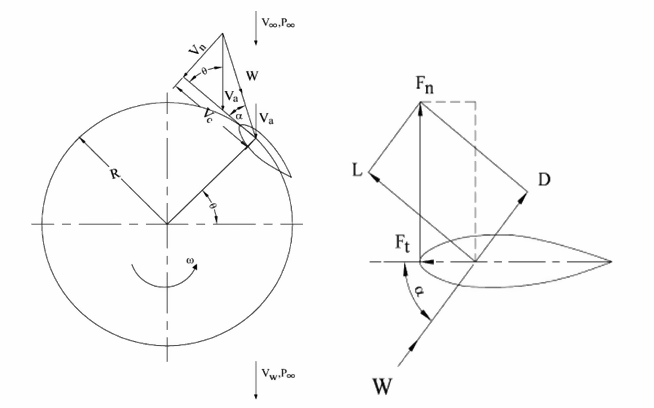
\includegraphics[width=0.9\textwidth, height=0.9\textheight, keepaspectratio=true]{media/image7837.png}
\caption{Flow velocities and force diagram of a single blade airfoil (Adapted from Mazharul Islam et al., 2008) \protect \label{fig:flow-velocities-and-force-diagram-of-a-single}}
\end{figure}

If tip speed ratio at the time step is greater than the maximum tip speed ratio, the model estimates actual rotor speed at the time step as:

\begin{equation}
\omega R = \lambda {V_{Local}}
\end{equation}

The model then employs general mathematical expressions for the aerodynamic analysis of straight-bladed Darrieus-type VAWTs to predict the power production by VAWTs. Assuming quasi-steady state, the induced wind speed (\emph{V\(_{a}\)}) on the rotor is defined as:

\begin{equation}
{V_a} = \frac{2}{3}{V_{Local}}
\end{equation}

The chordal velocity (\emph{V\(_{c}\)}), normal velocity (\emph{V\(_{n}\)}), and relative flow velocity (\emph{W}) as shown in figure above can be expressed as:

\begin{equation}
{V_c} = \omega R + {V_a}\cos \theta
\end{equation}

\begin{equation}
{V_n} = {V_a}\sin \theta
\end{equation}

\begin{equation}
W = \sqrt {V_c^2 + V_n^2}
\end{equation}

The expression for the non-dimensional angle of attack \(\alpha\) with no consideration of blade pitch is:

\begin{equation}
\alpha  = {\tan ^{ - 1}}\left[ {\frac{{\sin \theta }}{{{{(\omega R} \mathord{\left/ {\vphantom {{(\omega R} {{V_{Local}})/({{{V_a}} \mathord{\left/ {\vphantom {{{V_a}} {{V_{Local}}}}} \right. } {{V_{Local}}}}}}} \right. } {{V_{Local}})/({{{V_a}} \mathord{\left/ {\vphantom {{{V_a}} {{V_{Local}}}}} \right. } {{V_{Local}}}}}}) + \cos \theta }}} \right]
\end{equation}

The tangential and normal force coefficients, respectively, are expressed as:

\begin{equation}
{C_t} = {C_l}\sin \alpha  + {C_d}\cos \alpha
\end{equation}

\begin{equation}
{C_n} = {C_l}\cos \alpha  + {C_d}\sin \alpha
\end{equation}

The net tangential and normal forces are obtained from the following expressions:

\begin{equation}
{F_t} = {C_t}\frac{1}{2}{\rho_{Local}}{A_c}{W^2}
\end{equation}

\begin{equation}
{F_n} = {C_n}\frac{1}{2}{\rho_{Local}}{A_c}{W^2}
\end{equation}

Average tangential force on a single blade can be defined as:

\begin{equation}
{F_{ta}} = \frac{1}{{2\pi }}\int_0^{2\pi } {{F_t}(\theta )d\theta }
\end{equation}

Substituting the value of \emph{F\(_{t}\)} and arranging the tangential force on the azimuth angle, \(\theta\), the equation above can be written as:

\begin{equation}
{F_{ta}} = \frac{1}{{4\pi }}{C_t}{\rho_{Local}}{A_c}(\int_0^{2\pi } {{{(\omega R)}^2}}  + \int_0^{2\pi } {V_a^2} )
\end{equation}

The expression of the total torque for the number of blades is defined as:

\begin{equation}
Q = N{F_{ta}}
\end{equation}

The power production of wind turbine is thus:

\begin{equation}
{P_W} = Q\omega
\end{equation}

The model also defines \emph{P\(_{W}\)} as the rated power output at the rated wind speed, if either the power production of wind turbine or local wind speed is greater than the rated power.

The overall power production delivered from a wind turbine system is thus:

\begin{equation}
P = \eta {P_W}
\end{equation}

% table 92
\begin{longtable}[c]{p{1.2in}p{3.3in}p{1.5in}}
\caption{Nomenclature for Wind Turbine model \label{table:nomenclature-for-wind-turbine-model}} \tabularnewline
\toprule 
Variable & Description & Units \tabularnewline
\midrule
\endfirsthead

\caption[]{Nomenclature for Wind Turbine model} \tabularnewline
\toprule 
Variable & Description & Units \tabularnewline
\midrule
\endhead

A\(_{R}\) & swept area of rotor & m\(^{2}\) \tabularnewline
A\(_{C}\) & blade chord area & m\(^{2}\) \tabularnewline
a & site wind exponent, 0.22 & ~ \tabularnewline
a\(_{met}\) & wind exponent, 0.14 & ~ \tabularnewline
C\(_{d}\) & blade drag coefficient, 0.9 & ~ \tabularnewline
C\(_{l}\) & blade lift coefficients, 0.05 & ~ \tabularnewline
C\(_{n}\) & normal force coefficient & ~ \tabularnewline
C\(_{p}\) & power coefficient (performance coefficient) & ~ \tabularnewline
C\(_{t}\) & tangential force coefficient & ~ \tabularnewline
C\(_{1-6}\) & empirical power coefficient parameters & ~ \tabularnewline
g\(_{o}\) & standard gravity & m/s\(^{2}\) \tabularnewline
F\(_{n}\) & normal force in radial direction & N-m (J) \tabularnewline
F\(_{t}\) & tangential force & N-m (J) \tabularnewline
F\(_{ta}\) & average tangential force & N-m (J) \tabularnewline
F\(_{v}\) & wind speed factor & ~ \tabularnewline
H & height of local wind speed measurement & m \tabularnewline
H\(_{met}\) & height of turbine, 10 & m \tabularnewline
N & number of blade & ~ \tabularnewline
P & overall power production delivered to building~ & W \tabularnewline
P\(_{Local}\) & outdoor static air pressure at rotor height & Pa \tabularnewline
P\(_{W}\) & wind turbine power produced & W \tabularnewline
Q & overall torque & N-m \tabularnewline
R & turbine radius & m \tabularnewline
T\(_{Local}\) & local air temperature at rotor height & \(^{\circ}\)C \tabularnewline
v & ambient wind speed & m/s \tabularnewline
v\(_{1}\) & upstream wind speed & m/s \tabularnewline
v\(_{2}\) & wind speed on the turbine & m/s \tabularnewline
v\(_{3}\) & downstream wake velocity & m/s \tabularnewline
V\(_{a}\) & induced velocity & m/s \tabularnewline
V\(_{AnnualAvg}\) & annual average wind speed from TMY weather data & m/s \tabularnewline
V\(_{Local}\) & local wind speed at the location of the system & m/s \tabularnewline
V\(_{LocalTMY}\) & annual average wind speed converted at the local station height & m/s \tabularnewline
V\(_{c}\) & chordal velocity component & m/s \tabularnewline
V\(_{n}\) & normal velocity component & m/s \tabularnewline
V\(_{Z}\) & wind speed adjusted at rotor height & m/s \tabularnewline
W & relative flow velocity & m/s \tabularnewline
Z & height of wind turbine rotor & m \tabularnewline
$\alpha$ & blade angle of attack & deg \tabularnewline
$\theta$ & azimuth angle in VAWT and pitch angle in HAWT & deg \tabularnewline
$\rho$\(_{Local}\) & local density of air at rotor height & kg/m\(^{3}\) \tabularnewline
$\omega$ & angular velocity of turbine & rad/s \tabularnewline
$\omega$\(_{Local}\) & local humidity ratio at rotor height & kg-H\(_{2}\)O/kg-air \tabularnewline
x & exponent, 1.5 & ~ \tabularnewline
$\lambda$ & tip speed ratio & ~ \tabularnewline
$\lambda$\(_{i}\) & tip speed ratio at the i\(^{th}\) pitch & ~ \tabularnewline
$\delta$\(_{met}\) & wind boundary layer thickness of meteorological station, 270 & m \tabularnewline
$\delta$ & site boundary layer thickness, 370 & m \tabularnewline
$\eta$ & wind turbine system efficiency & ~ \tabularnewline
\bottomrule
\end{longtable}

\subsubsection{References}\label{references-3-002}

Siegfried Heier. 2006. Grid Integration of Wind Energy Conversion Systems, Second Edition. Wiley, Chap. 2, pp.31-44.

Mazharul Islam, David S.K. Ting and Amir Fartaj. 2008. Aerodynamic Models for Darrieus-type Sraight-bladed Vertical Axis Wind Turbines. Renewable \& Sustainable Energy Reviews, Volume 12, pp.1087-1109.

ASHRAE. 2005. Handbook of Fundamentals, pp 16.3-16.4, Atlanta: ASHRAE.
